\documentclass[12pt,letterpaper]{article}
\usepackage{graphicx,textcomp}
\usepackage{natbib}
\usepackage{setspace}
\usepackage{fullpage}
\usepackage{color}
\usepackage[reqno]{amsmath}
\usepackage{amsthm}
\usepackage{fancyvrb}
\usepackage{amssymb,enumerate}
\usepackage[all]{xy}
\usepackage{endnotes}
\usepackage{lscape}
\newtheorem{com}{Comment}
\usepackage{float}
\usepackage{hyperref}
\newtheorem{lem} {Lemma}
\newtheorem{prop}{Proposition}
\newtheorem{thm}{Theorem}
\newtheorem{defn}{Definition}
\newtheorem{cor}{Corollary}
\newtheorem{obs}{Observation}
\usepackage[compact]{titlesec}
\usepackage{dcolumn}
\usepackage{tikz}
\usetikzlibrary{arrows}
\usepackage{multirow}
\usepackage{xcolor}
\newcolumntype{.}{D{.}{.}{-1}}
\newcolumntype{d}[1]{D{.}{.}{#1}}
\definecolor{light-gray}{gray}{0.65}
\usepackage{url}
\usepackage{listings}
\usepackage{color}

\definecolor{codegreen}{rgb}{0,0.6,0}
\definecolor{codegray}{rgb}{0.5,0.5,0.5}
\definecolor{codepurple}{rgb}{0.58,0,0.82}
\definecolor{backcolour}{rgb}{0.95,0.95,0.92}

\lstdefinestyle{mystyle}{
	backgroundcolor=\color{backcolour},  
	commentstyle=\color{codegreen},
	keywordstyle=\color{magenta},
	numberstyle=\tiny\color{codegray},
	stringstyle=\color{codepurple},
	basicstyle=\footnotesize,
	breakatwhitespace=false,        
	breaklines=true,                
	captionpos=b,                    
	keepspaces=true,                
	numbers=left,                    
	numbersep=5pt,                  
	showspaces=false,                
	showstringspaces=false,
	showtabs=false,                  
	tabsize=2
}
\lstset{style=mystyle}
\newcommand{\Sref}[1]{Section~\ref{#1}}
\newtheorem{hyp}{Hypothesis}

\title{Problem Set 2}
\date{Due: October 22, 2026}
\author{Applied Stats/Quant Methods 1}

\begin{document}
	\maketitle
	\section*{Instructions}
	\begin{itemize}
		\item Please show your work! You may lose points by simply writing in the answer. If the problem requires you to execute commands in \texttt{R}, please include the code you used to get your answers. Please also include the \texttt{.R} file that contains your code. If you are not sure if work needs to be shown for a particular problem, please ask.
		\item Your homework should be submitted electronically on GitHub.
		\item This problem set is due before 23:59 on Thursday October 22, 2026. No late assignments will be accepted.
		
	\end{itemize}
	
	
	\vspace{.5cm}
	\section*{Question 1: Political Science}
	\vspace{.25cm}
	The following table was created using the data from a study run in a major Latin American city.\footnote{Fried, Lagunes, and Venkataramani (2010). ``Corruption and Inequality at the Crossroad: A Multimethod Study of Bribery and Discrimination in Latin America. \textit{Latin American Research Review}. 45 (1): 76-97.} As part of the experimental treatment in the study, one employee of the research team was chosen to make illegal left turns across traffic to draw the attention of the police officers on shift. Two employee drivers were upper class, two were lower class drivers, and the identity of the driver was randomly assigned per encounter. The researchers were interested in whether officers were more or less likely to solicit a bribe from drivers depending on their class (officers use phrases like, ``We can solve this the easy way'' to draw a bribe). The table below shows the resulting data.
	
	\newpage
	\begin{table}[h!]
		\centering
		\begin{tabular}{l | c c c }
			& Not Stopped & Bribe requested & Stopped/given warning \\
			\\[-1.8ex]
			\hline \\[-1.8ex]
			Upper class & 14 & 6 & 7 \\
			Lower class & 7 & 7 & 1 \\
			\hline
		\end{tabular}
	\end{table}
	
	\begin{enumerate}
		
		\item [(a)]
		Calculate the $\chi^2$ test statistic by hand/manually (even better if you can do "by hand" in \texttt{R}).\\
		\vspace{.5cm}
		
		We formulate two hypotheses: \\
		H0: the variables are statistically independent from each other.\\
		H1: the variables are statistically dependent from each other.\\
		
		In order to calculate the $\chi^2$ test statistic, we need to calculate the expected frequency corresponding to each observed frequency in the table. The result will in turn allow us to calculate the $\chi^2$ test statistic for each cell. As a reminder, the formula is the following (with $F_E$ the expected frequency and $F_O$ the observed frequency):
		\[
		F_E = \frac{\text{row total}}{\text{grand total}} * {\text{column total}}
		\]
		 \\
		\[ \chi^2 = \frac{sum(F_O - F_E)^2}{F_E}
		\]
		
		
		For the upper class drivers:
		
		\lstinputlisting[language=R, firstline=66, lastline=73]{PS02_answers_NF.R}  
		
		
		Result:
		\lstinputlisting[language=R, firstline=78, lastline=79]{PS02_answers_NF.R}  
		
		\begin{verbatim}
			> print(Chi_square_upper)
			[1] 1.353989
		\end{verbatim}
		
		\vspace{.2cm}
		
		For the lower class drivers:
		
		\lstinputlisting[language=R, firstline=83, lastline=90]{PS02_answers_NF.R}  
		Result:
		\lstinputlisting[language=R, firstline=92, lastline=93]{PS02_answers_NF.R}  
		\begin{verbatim}
			> print(Chi_square_lower)
			[1] 2.437179
		\end{verbatim}
		
		Now we can easily calculate the $\chi^2$ test statistic, by adding the $\chi^2$ of the upper cells and the lower cells:
		Result:
		\lstinputlisting[language=R, firstline=96, lastline=97]{PS02_answers_NF.R}  
		\begin{verbatim}
			> print(Chi_square)
			[1] 3.791168
		\end{verbatim}
		
		
		
		\vspace{.2cm}
		\item [(b)]
		Now calculate the p-value from the test statistic you just created (in \texttt{R}).\footnote{Remember frequency should be $>$ 5 for all cells, but let's calculate the p-value here anyway.}  What do you conclude if $\alpha = 0.1$?\\
		
		We calculate the p-value using R commands and the degrees of freedom:
		\lstinputlisting[language=R, firstline=103, lastline=105]{PS02_answers_NF.R}  
		\newpage
		Result:
		\begin{verbatim}
			> df
			[1] 2
			> pchisq(Chi_square, df=2, lower.tail=F)
			[1] 0.1502306
		\end{verbatim}
		Our p-value is 0.15\textgreater0.1. From this, we conclude that we fail to reject the null hypothesis according to which both variables are statistically independent from each other. Thus, we do not have sufficient evidence to say that there is an association between our variables.
		
		
		\vspace{1cm}
		\item [(c)] Calculate the standardized residuals for each cell and put them in the table below. \\
		
		As a reminder, this is the formula for standardised residuals: \\
		$$z = \frac{F_O - F_E}{SE} = \frac{F_O - F_E}{\sqrt{F_E * (1-(\text{row total}/\text{total}))*(1-(\text{column total}/\text{total}))}} $$ \\
		
		Here are the calculations for each cell:
		\lstinputlisting[language=R, firstline=114, lastline=132]{PS02_answers_NF.R}
		The filled table looks like this:
		
		
		\begin{table}[h]
			\centering
			\begin{tabular}{l | c c c }
				& Not Stopped & Bribe requested & Stopped/given warning \\
				\\[-1.8ex]
				\hline \\[-1.8ex]
				Upper class  & 0.322 & -1.642 & 1.523 \\
				
				Lower class & -0.322
				& 1.642  & -1.523  \\
				
			\end{tabular}
		\end{table}
		
		
		\vspace{1cm}
		\item [(d)] How might the standardized residuals help you interpret the results?  \\
		The closer to 0 a standardised residual is, the more it supports the null hypothesis: the cells with the highest standardised residuals therefore are the ones that make the biggest contribution. In this case, it is drivers of the lower class who encoutered an agent asking for a bribe, and drivers of the upper class who were only stopped. It does support the theoretical argument made in the paper that states that drivers who are perceived by the police to be of a lower class will more often be asked to pay a bribe, because they are seen as better targets by corrupt officials. On the contrary, drivers who are perceived as being of the upper class will more often be let go with no issue. This is on average, and for similar infractions.
		
	\end{enumerate}
	\newpage
	
	\section*{Question 2: Economics}
	Chattopadhyay and Duflo were interested in whether women promote different policies than men.\footnote{Chattopadhyay and Duflo. (2004). ``Women as Policy Makers: Evidence from a Randomized Policy Experiment in India. \textit{Econometrica}. 72 (5), 1409-1443.} Answering this question with observational data is pretty difficult due to potential confounding problems (e.g. the districts that choose female politicians are likely to systematically differ in other aspects too). Hence, they exploit a randomized policy experiment in India, where since the mid-1990s, $\frac{1}{3}$ of village council heads have been randomly reserved for women. A subset of the data from West Bengal can be found at the following link: \url{https://raw.githubusercontent.com/kosukeimai/qss/master/PREDICTION/women.csv}\\
	
	\noindent Each observation in the data set represents a village and there are two villages associated with one GP (i.e. a level of government is called "GP"). Figure~\ref{fig:women_desc} below shows the names and descriptions of the variables in the dataset. The authors hypothesize that female politicians are more likely to support policies female voters want. Researchers found that more women complain about the quality of drinking water than men. You need to estimate the effect of the reservation policy on the number of new or repaired drinking water facilities in the villages.
	\vspace{.5cm}
	\begin{figure}[h!]
	\caption{\footnotesize{Names and description of variables from Chattopadhyay and Duflo (2004).}}
	\vspace{.5cm}
	\centering
	\label{fig:women_desc}
	\includegraphics[width=1.1\textwidth]{../../../../graphics/women_desc.png}
	\end{figure}
	
	\newpage
	\vspace{1cm}
	\begin{enumerate}
		\item [(a)] State a null and alternative (two-tailed) hypothesis.
		
		Researchers hypothesize that female politicians are more likely to support policies female voters want. They have found that more women complain about the quality of drinking water than men.
		We can hypothesise from this that female politicians are more likely to push for newer/repaired drinking facilities in the villages, which will in turn increase the number of such drinking facilities. We are therefore looking for a correlation between both variables (Pearson's r). \\
		
		H0: there is no correlation, or linear association, between X and Y. \\
		H1: there is a correlation, or linear association, between X and Y. \\
		
		
		\vspace{1cm}
		\item [(b)] Run a bivariate regression to test this hypothesis in \texttt{R} (include your code!).
		
		We start by looking at our data to try and observe the association.
		\lstinputlisting[language=R, firstline=160, lastline=163]{PS02_answers_NF.R}
		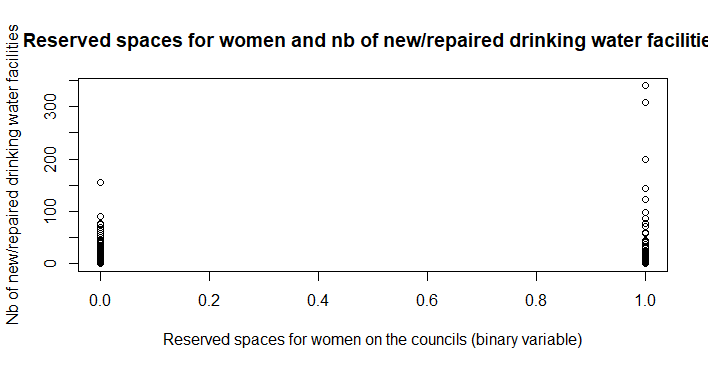
\includegraphics[width=1\linewidth,height=.5\textheight,keepaspectratio]{Plot q2}
		It seems that there are more/newer repaired drinking water facilities (higher Y values) when women have reserved spaces on councils (X=1).
		
		Then we calculate the correlation coefficient:
		\lstinputlisting[language=R, firstline=168, lastline=169]{PS02_answers_NF.R}
		
		\vspace{.5cm}
		\item [(c)] Interpret the coefficient estimate for reservation policy. \\
		We get a correlation coefficient of 0.12, which is quite small: there is almost no linear association between both. However, this may be because we are dealing with a binary variable.  \\
		We do get a p-value of 0.01\textless0.05 (for a 95\% confidence interval), which indicates that the results are significant. It does not say anything on the strength of the association, though, and thus does not change our interpretation. \\
		On average, when there are no spaces reserved for women on councils (X=0), there are around 14 new or repaired water facilities. Every one unit increase of X is associated with a 9.2 increase in Y on average.
		
		\end{enumerate}
		
\end{document}